\documentclass[parskip=full]{scrartcl}
\usepackage[utf8]{inputenc}
\usepackage[T1]{fontenc}
\usepackage{lmodern}
\usepackage{amsmath}
\usepackage{graphicx, subfigure}
\usepackage{array}
\usepackage{caption}
\usepackage[noabbrev]{cleveref}
%\usepackage[crop=off]{auto-pst-pdf} % pdf-figs machen sonst probleme

\usepackage[numbers]{natbib}

\usepackage{listings}

\usepackage{shorttoc}
\usepackage{etoolbox}
\usepackage{float}

\usepackage[para]{footmisc}

\usepackage{epstopdf}
\epstopdfDeclareGraphicsRule{.tif}{png}{.png}{convert #1 \OutputFile}
\AppendGraphicsExtensions{.tif}

\usepackage{url}
\usepackage{xcolor}
\definecolor{javared}{rgb}{0.6,0,0} % for strings
\definecolor{javagreen}{rgb}{0.25,0.5,0.35} % comments
\definecolor{javapurple}{rgb}{0.5,0,0.35} % keywords
\definecolor{javadocblue}{rgb}{0.25,0.35,0.75} % javadoc
\usepackage{listings}
\usepackage{caption}
\DeclareCaptionFont{white}{\color{white}}
\DeclareCaptionFormat{listing}{%
  \parbox{\textwidth}{\colorbox{gray}{\parbox{\textwidth}{#1#2#3}}\vskip-4pt}}
\captionsetup[lstlisting]{format=listing,labelfont=white,textfont=white}
\lstset{frame=lrb,xleftmargin=\fboxsep,xrightmargin=-\fboxsep,
language=Java,
basicstyle=\ttfamily,
keywordstyle=\color{javapurple}\bfseries,
stringstyle=\color{javared},
commentstyle=\color{javagreen},
morecomment=[s][\color{javadocblue}]{/**}{*/},
numbers=left,
numberstyle=\tiny\color{black},}


 
\title{Specifications for Extraction of Implicit User Rating from BBC Data Set}


\subject{University of Zurich, Department of Informatics\\Report P2P Challenge Task 2013 Team 3}

\date{14. June 2013}


\graphicspath{ {./figures/} }


\author{Fabian Christoffel\footnote{fabian.christoffel@uzh.ch}}
\begin{document}

\pagenumbering{roman}
We want to obtain implicit user ratings for a TV program based on the users consumption behavior. From the BBC data set the percentage of a TV show watched by a user is readily available from column 3 of the CSV file (aggregation:totalUserProgramFraction). However, I think we can obtain a better estimate of the users interest in a TV program than just using this percentage by considering the 'locality' of the watched time span within the total time span of the TV program:
\begin{itemize}
	\item \textit{Program is watched from the beginning but not to the end:} We can argue that a user who watched a TV show from the very beginning, had an a priori expectation of the shows high quality (from its own perspective) and hence decided to watch the entire show beforehand. If the user tuned out prematurely we can assume that the quality of the program did not meet the users expectations. For this reason we do not map the rating linearly to the percentage of the watched program but with a positive curvature (see red graph in figure~\ref{fig:kurven}).
	\item \textit{Program is watched to the end but not from the beginning:} In this case we can assume that the user was not aware of the program or did not know it at all. Hence, the interest of the user in the program could actually be high, even though the user watched only a short time span of the entire program. For this reason we map the watched program share to the user rating with a negative curvature (see blue graph in figure~\ref{fig:kurven}).
\end{itemize}

\begin{figure}[h!]
   \centering
      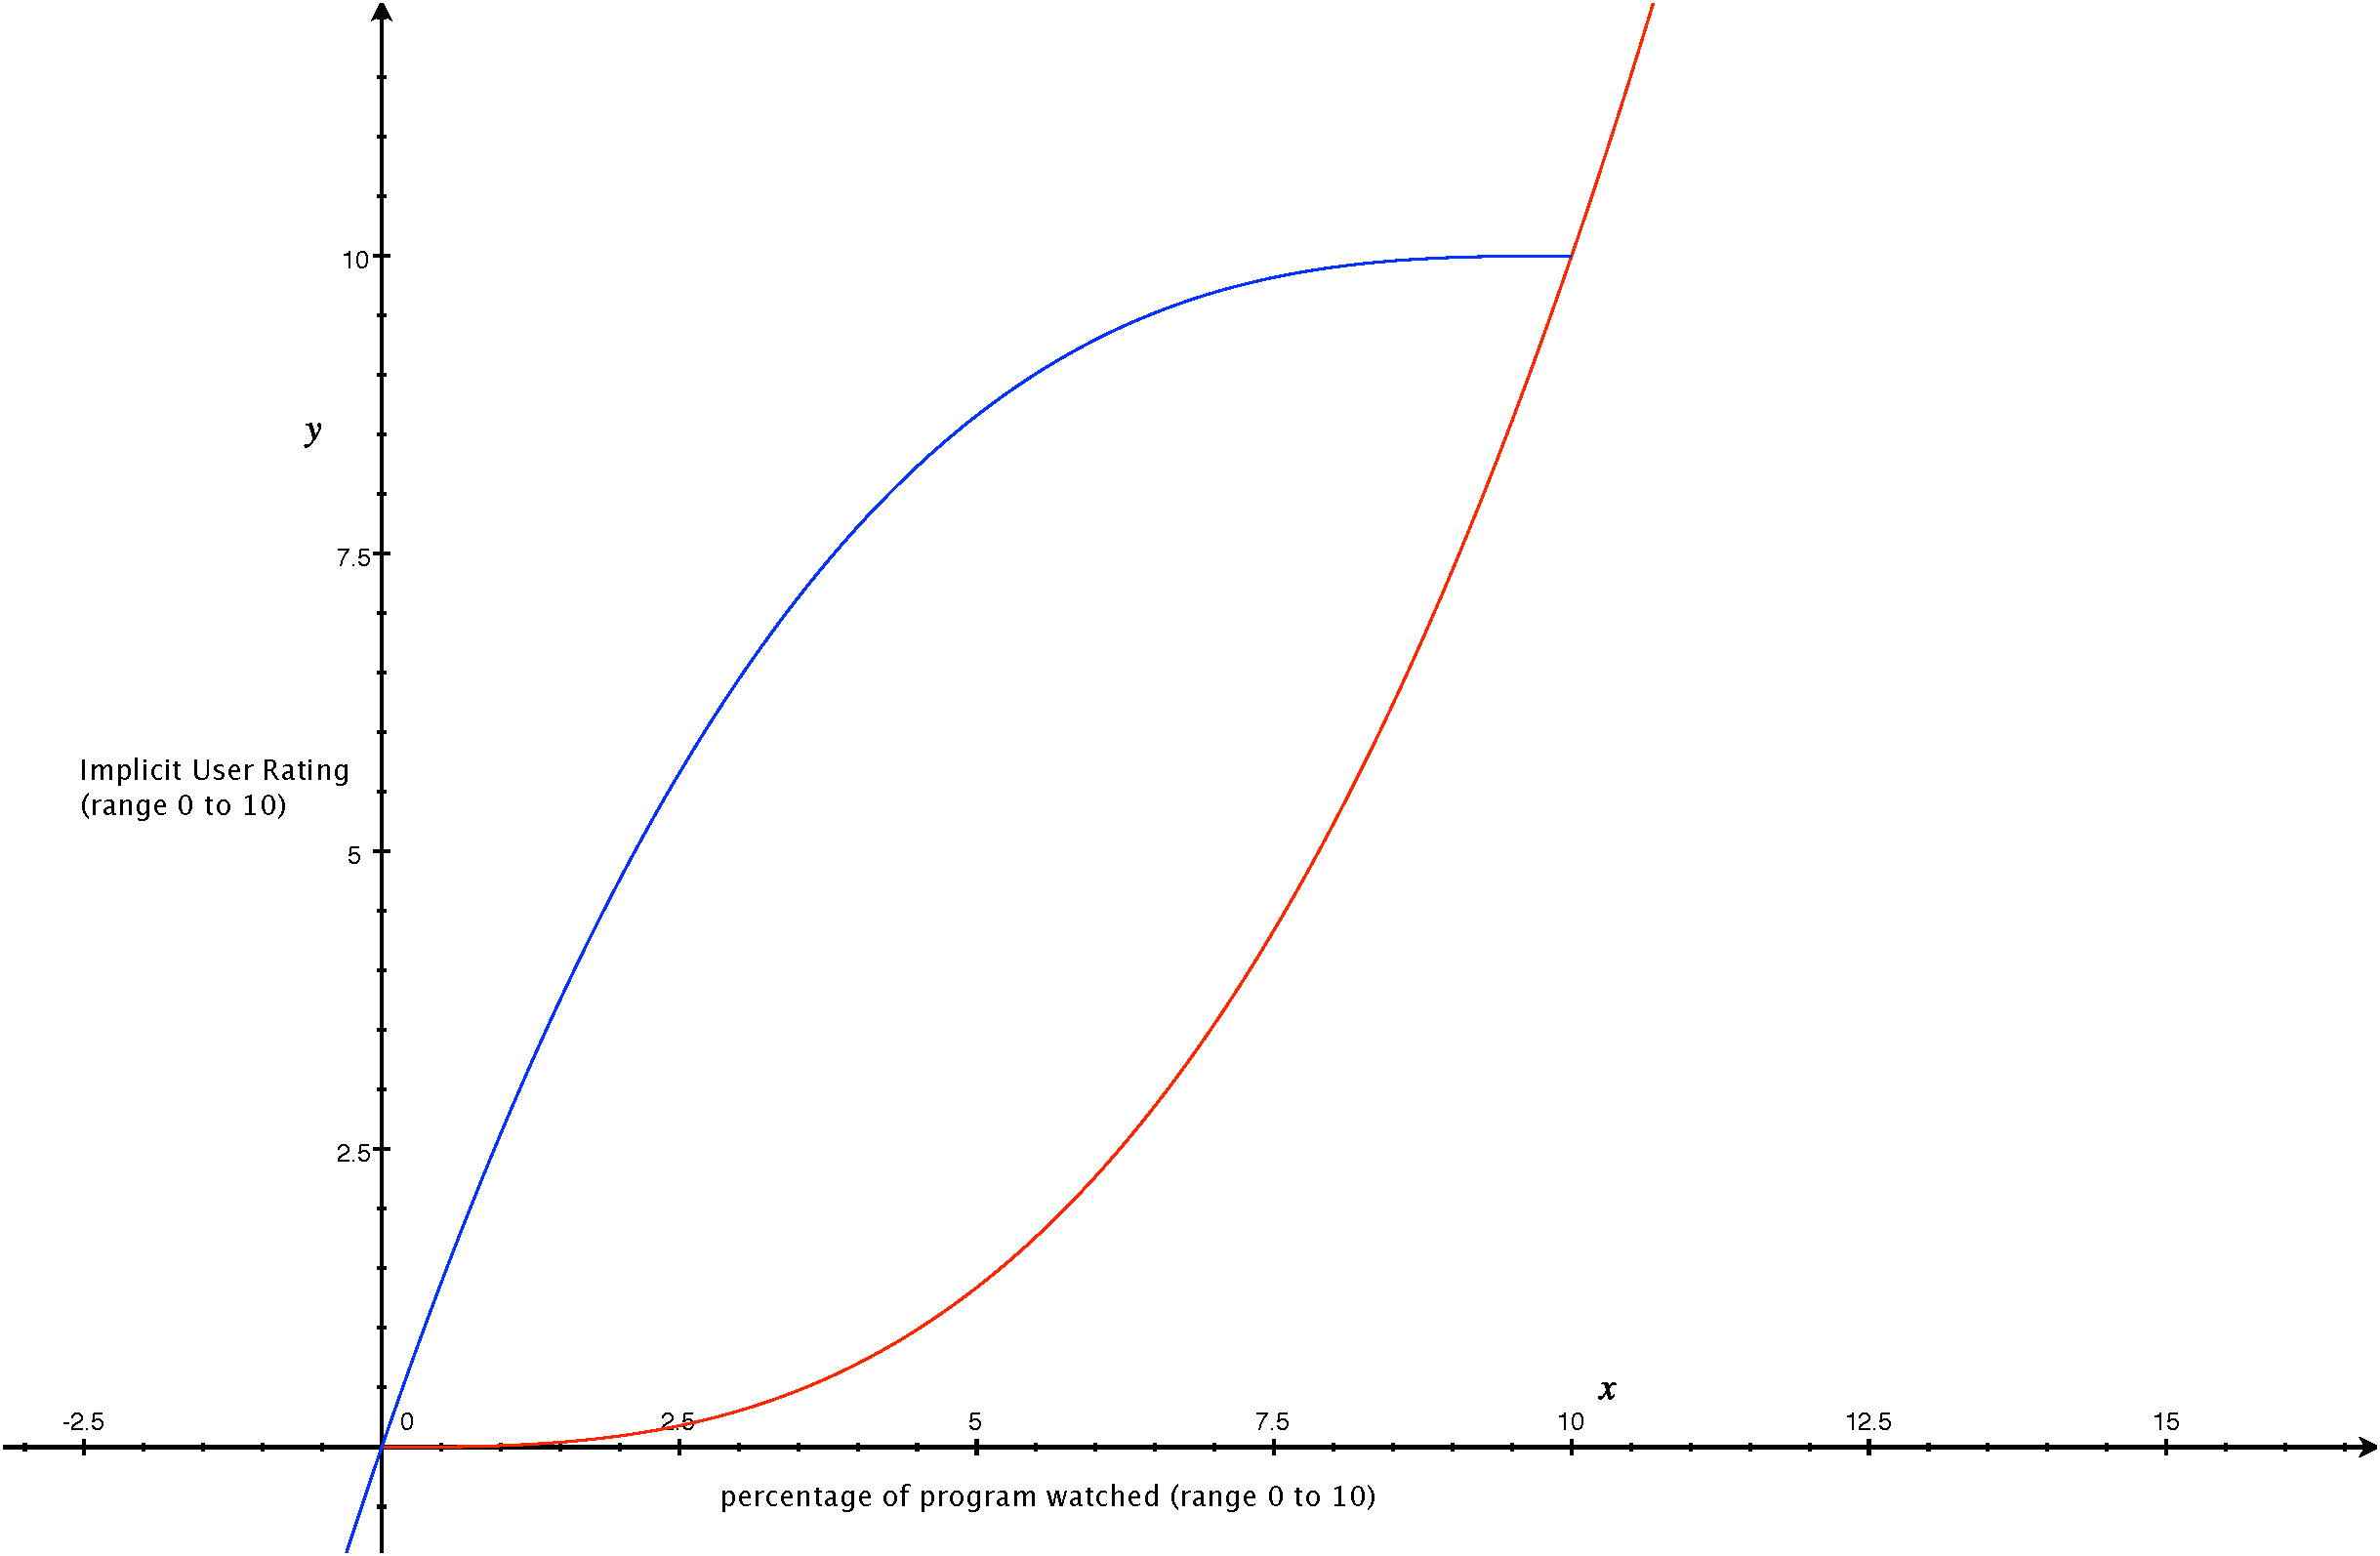
\includegraphics[width=0.75\textwidth]{kurven2}
   \caption{In red: watched share user rating mapping for premature termination. In blue: watched share user rating mapping for delayed tune in.}
   \label{fig:kurven}
\end{figure}

The afore-mentioned considerations can be translated into a simple algorithm (see listing~\ref{listing:main}), where \texttt{$p_{1}$} and \texttt{$p_{2}$} adjust the curvature as desired by the user. The share of TV program watched is in the range of 0 to 1 and we want to obtain a user interest rating in the range of o to 10.

\begin{lstlisting}[mathescape, breaklines=true,label=listing:main,caption=Main method for implicit user rating generation.]

double getImplicitRating(UsageDataSetEntry entry) {

	double percentageWatched <- entry.get("aggregation:totalUserProgramFraction") * 10; // is in range 0-1 in data set

	boolean fromBeginning <- watchedFromBeginningOfProgram(entry);
	boolean tillEnd <- watchedTillEndOfProgram(entry);

	if (fromBeginning && tillEnd)
		return percentageWatched;

	if (fromBeginning)
		return $\displaystyle \frac{percentageWatched^{p_{1}}}{10^{p_{1}-1}};$
	
	if (tillEnd)
		return $\displaystyle 10-\frac{(10-percentageWatched)^{p_{2}}}{10^{p_{2}-1}};$

	return percentageWatched;
}
\end{lstlisting}

\begin{lstlisting}[mathescape, breaklines=true,label=listing:watchedFromBeginningOfProgram,caption=Method watchedFromBeginningOfProgram.]

boolean watchedFromBeginningOfProgram(UsageDataSetEntry entry) {

	long epgStartTime <- epgData.get(entry.get("epg:id")).get("epg:start"); // in seconds since start of epoch
	
	long userStartTime <- entry.get("program_session:start_time"); // in seconds since start of epoch
	
	double tolerance <- entry.get("epg:duration"); // in seconds
	tolerance <- (tolerance * START_TIME_TOLERANCE_PERCENTAGE) / 100.0;
	
	if (epgStartTime + tolerance >= userStartTime)
		return true;

	return false;
}
\end{lstlisting}

\begin{lstlisting}[mathescape, breaklines=true,label=listing:watchedTillEndOfProgram,caption=Method watchedTillEndOfProgram.]

boolean watchedTillEndOfProgram(UsageDataSetEntry entry) {

	long epgEndTime <- epgData.get(entry.get("epg:id")).get("epg:end"); // in seconds since start of epoch
	
	long userEndTime <- entry.get("program_session:start_time"); // in seconds since start of epoch
	userEndTime <- userEndTime + entry.get("program_session:duration"); // in seconds
	
	double tolerance <- entry.get("epg:duration"); // in seconds
	tolerance <- (tolerance * END_TIME_TOLERANCE_PERCENTAGE) / 100.0;
	
	if (epgEndTime - tolerance <= userEndTime)
		return true;

	return false;
}
\end{lstlisting}



\end{document}